
\pdfminorversion=4

% Modos:
% Definir el comando \handoutmode como "1" para compilar las diapositivas en
% modo handout
% al pdf generado ejecutarle el siguiente comando para poner varias diapo en una misma pagina:
%    pdfnup FILE.pdf --nup 2x3 --no-landscape --paper letterpaper --frame True
%
% Definir \handoutmode como algo distinto de "1" para compilar las diapositivas
% normalmente.
%
% Para configurar el modo desde afuera (la linea de comandos de latex) correr
% la compilacion como:
%
%   latex -output-directory=tmp -output-format=pdf '\def\handoutmode{1}\include{FILE.tex}'
%
\if\handoutmode1
    \documentclass[professionalfonts,handout]{beamer}
    \setbeameroption{show notes}
    \setbeamertemplate{note page}{\insertnote}
    \setbeamercolor{background canvas}{bg=white}
\else
    \documentclass[professionalfonts]{beamer}
\fi


% Template original the Beamer: Copyright 2004 by Till Tantau <tantau@users.sourceforge.net>.


\mode<presentation>
{
  \usetheme{metropolis}
  % or ...

  %\setbeamercovered{transparent} %hace que lo que esta covered se muestre transparente
}

\setbeamertemplate{navigation symbols}{}%remove navigation symbols

\usepackage[english]{babel}

\usepackage[latin1]{inputenc}

\usepackage{times}
\usepackage[T1]{fontenc}

% para poder escribir codigo fuente en las diapositivas
\usepackage{listings}

% para graficar diagramas simples y arboles de jerarquias
\usepackage{tikz}
\usepackage{tikz-qtree}
\usetikzlibrary{matrix,positioning}
\usetikzlibrary{shapes,arrows,chains,calc,decorations.pathmorphing}

\usepackage{xcolor}
\definecolor{darkgreen}{rgb}{0,.5,0}
\definecolor{darkblue}{rgb}{0,0,.7}
\lstdefinestyle{normal}{language=C++,       % lenguaje C++
   numbers=left,                            % enumerar las lineas
   keywordstyle=\color{darkblue}\textbf,    % color de las keywords
   stringstyle=\color{red},                 % color de los strings
   commentstyle=\color{darkgreen},          % color de los comentarios
   basicstyle=\color{black}\ttfamily\footnotesize\bfseries,     % color del texto en general
   morecomment=[l][\color{magenta}]{\#},    % coloreamos las intrucciones del precompilador (todo lo que empieza con #)
   ndkeywords={NULL,nullptr,siz,zer,mov,add},               % definimos una nuevas keywords como NULL y nullptr
   ndkeywordstyle=\color{violet},           % y las nuevas keywords tendran este color
   frame=simple,                            % simple, sin ningun marco o frame alrededor del codigo
   basewidth={0.55em,0.55em}                % tamano de las letras/lineas. usado para reducir el whitespace entre estas
}

\lstdefinestyle{normal33}{language=C++,       % lenguaje C++
   numbers=left,                            % enumerar las lineas
   keywordstyle=\color{darkblue}\textbf,    % color de las keywords
   stringstyle=\color{red},                 % color de los strings
   commentstyle=\color{darkgreen},          % color de los comentarios
   basicstyle=\color{black}\ttfamily\footnotesize\bfseries,     % color del texto en general
   morecomment=[l][\color{magenta}]{\#},    % coloreamos las intrucciones del precompilador (todo lo que empieza con #)
   ndkeywords={NULL,nullptr},               % definimos una nuevas keywords como NULL y nullptr
   ndkeywordstyle=\color{violet},           % y las nuevas keywords tendran este color
   frame=simple,                            % simple, sin ningun marco o frame alrededor del codigo
   basewidth={0.55em,0.55em}                % tamano de las letras/lineas. usado para reducir el whitespace entre estas
}
%mismo estilo, sin numeros
\lstdefinestyle{normalnonumbers}{language=C++,
   keywordstyle=\color{darkblue}\textbf,
   stringstyle=\color{red},           
   commentstyle=\color{darkgreen},    
   basicstyle=\color{black}\ttfamily\footnotesize\bfseries,
   morecomment=[l][\color{magenta}]{\#},
   ndkeywords={NULL,nullptr,move,add},          
   ndkeywordstyle=\color{violet}, 
   frame=simple,
   basewidth={0.55em,0.55em}
}


% mismo estilo pero todos los colores estan mas debiles como si se volvieran transparentes
% usado para poder resaltar el codigo.
\lstdefinestyle{dimmided}{language=C++,
   keywordstyle=\color{darkblue!30}\textbf,
   stringstyle=\color{red!30},
   commentstyle=\color{darkgreen!30},
   basicstyle=\color{black!30}\ttfamily\footnotesize\bfseries,
   morecomment=[l][\color{magenta!30}]{\#},
   ndkeywords={NULL,nullptr,siz,zer,mov,add},
   ndkeywordstyle=\color{violet!30}, 
   moredelim=**[is][\only<+->{\color{black}\lstset{style=normal}}]{@}{@}, % definimos que las lineas entre arrobas (@) tendran el estilo normal (con los colores a toda intensidad)
   frame=simple,
   basewidth={0.55em,0.55em}
}
\lstdefinestyle{dimmided42}{language=C++,
   keywordstyle=\color{darkblue!30}\textbf,
   stringstyle=\color{red!30},
   commentstyle=\color{darkgreen!30},
   basicstyle=\color{black!30}\ttfamily\footnotesize\bfseries,
   morecomment=[l][\color{magenta!30}]{\#},
   ndkeywords={NULL,nullptr,siz,zer,mov,add},
   ndkeywordstyle=\color{violet!30}, 
   moredelim=**[is][{\color{black}\lstset{style=normal}}]{@}{@}, % definimos que las lineas entre arrobas (@) tendran el estilo normal (con los colores a toda intensidad)
   frame=simple,
   basewidth={0.55em,0.55em}
}

\lstdefinelanguage{json}{
    literate=
     *{:}{{{\color{violet}{:}}}}{1}
      {,}{{{\color{violet}{,}}}}{1}
      {\{}{{{\color{darkgreen}{\{}}}}{1}
      {\}}{{{\color{darkgreen}{\}}}}}{1}
      {[}{{{\color{darkgreen}{[}}}}{1}
      {]}{{{\color{darkgreen}{]}}}}{1},
}


\lstdefinestyle{normaljson}{language=json,  % lenguaje json
   numbers=left,                            % enumerar las lineas
   keywordstyle=\color{darkblue}\textbf,    % color de las keywords
   stringstyle=\color{red},                 % color de los strings
   commentstyle=\color{red},                % color de los comentarios
   basicstyle=\color{black}\ttfamily\footnotesize\bfseries,     % color del texto en general
   morecomment=[l][\color{magenta}]{\#},    % coloreamos las intrucciones del precompilador (todo lo que empieza con #)
   ndkeywords={NULL,nullptr},               % definimos una nuevas keywords como NULL y nullptr
   ndkeywordstyle=\color{violet},           % y las nuevas keywords tendran este color
   frame=simple,                            % simple, sin ningun marco o frame alrededor del codigo
   basewidth={0.55em,0.55em}                % tamano de las letras/lineas. usado para reducir el whitespace entre estas
}

\lstdefinelanguage{http}{
    morekeywords={
        GET,
        PUT,
        POST,
        DELETE
    }
}

\lstdefinestyle{normalhttp}{language=http,  % lenguaje HTTP
   numbers=left,                            % enumerar las lineas
   keywordstyle=\color{darkblue}\textbf,    % color de las keywords
   stringstyle=\color{red},                 % color de los strings
   commentstyle=\color{red},                % color de los comentarios
   basicstyle=\color{black}\ttfamily\footnotesize\bfseries,     % color del texto en general
   morecomment=[l][\color{magenta}]{\#},    % coloreamos las intrucciones del precompilador (todo lo que empieza con #)
   ndkeywords={NULL,nullptr},               % definimos una nuevas keywords como NULL y nullptr
   ndkeywordstyle=\color{violet},           % y las nuevas keywords tendran este color
   frame=simple,                            % simple, sin ningun marco o frame alrededor del codigo
   basewidth={0.55em,0.55em}                % tamano de las letras/lineas. usado para reducir el whitespace entre estas
}

% Pone las constantes numericas con color (violeta en este caso):
% - los numeros que estan dentro de un string/comentarios NO son coloreados
% - los numeros por fuera que pertenecen a una palabra SON coloreados 
%   (buf1, por ejemplo, el "1" es coloreado cuando no lo deberias. UPS!!)
% - No incluye el signo
% 
%\lstset{literate=%
%  *{0}{{{\color{violet}0}}}1
%   {1}{{{\color{violet}1}}}1
%   {2}{{{\color{violet}2}}}1
%   {3}{{{\color{violet}3}}}1
%   {4}{{{\color{violet}4}}}1
%   {5}{{{\color{violet}5}}}1
%   {6}{{{\color{violet}6}}}1
%   {7}{{{\color{violet}7}}}1
%   {8}{{{\color{violet}8}}}1
%   {9}{{{\color{violet}9}}}1
%}

% Para resaltar lineas de codigo usando \btLstHLB{range} y \btLstHLB<overlay>{range}:
% Por ejemplo, 
%  \btLstHLB{3}       linea 3 resaltada
%  \btLstHLB{1-5}     lineas de la 1 a la 5 resaltadas
%  \btLstHLB<2>{3}    linea 3 resaltada solo en el slide 2
%
% \btLstHLB usa un color azul mientras que \btLstHLR usa un color rojo como fondo
\usepackage{lstlinebgrd}
\makeatletter
\newcount\bt@rangea
\newcount\bt@rangeb

\newcommand\btIfInRange[2]{%
   \global\let\bt@inrange\@secondoftwo%
   \edef\bt@rangelist{#2}%
   \foreach \range in \bt@rangelist {%
      \afterassignment\bt@getrangeb%
      \bt@rangea=0\range\relax%
      \pgfmathtruncatemacro\result{ ( #1 >= \bt@rangea) && (#1 <= \bt@rangeb) }%
      \ifnum\result=1\relax%
      \breakforeach%
      \global\let\bt@inrange\@firstoftwo%
      \fi%
   }%
   \bt@inrange%
}
\newcommand\bt@getrangeb{%
   \@ifnextchar\relax%
   {\bt@rangeb=\bt@rangea}%
   {\@getrangeb}%
}
\def\@getrangeb-#1\relax{%
   \ifx\relax#1\relax%
      \bt@rangeb=100000%   \maxdimen is too large for pgfmath
   \else%
      \bt@rangeb=#1\relax%
   \fi%
}

%%%%%%%%%%%%%%%%%%%%%%%%%%%%%%%%%%%%%%%%%%%%%%%%%%%%%%%%%%%%%%%%%%%%%%%%%%%%%%
%
% \btLstHL<overlay spec>{range list}
%
\newcommand<>{\btLstHLB}[1]{%
   \only#2{\btIfInRange{\value{lstnumber}}{#1}{\color{blue!30}}% blue
   {\def\lst@linebgrdcmd####1####2####3{}}}%
}%
\newcommand<>{\btLstHLR}[1]{%
   \only#2{\btIfInRange{\value{lstnumber}}{#1}{\color{red!30}}% red
   {\def\lst@linebgrdcmd####1####2####3{}}}%
}%
%
%
%%%%%%%%%%%%%%%%%%%%%%

\makeatother


% sin fecha
\date{}

\author[7542]{Di Paola Mart\'in \\ \texttt{martinp.dipaola <at> gmail.com} }

\institute[Universidad de Buenos Aires]
{
   Facultad de Ingenier\'ia\\
   Universidad de Buenos Aires
}

% Definimos una imagen para que este en cada slide
%\pgfdeclareimage[height=0.5cm]{university-logo}{imgs/fiuba.png}
%\logo{\pgfuseimage{university-logo}}

%% Definir estas en el documento final
%%
%% \title%
%% {Programaci\'on gen\'erica y templates en C++}
%%
%% \subject{Programaci\'on gen\'erica y templates en C++}


%%%%%
% At begin of each Section do nothing; at each Subsection show the Section and Subsection names
% If the Section doesn't have a Subsection, then YOU must to add a unnumbered Subsection like \subsection*{}
% so the AtBeginSubsection will get triggered
\AtBeginSection{}
\AtBeginSubsection[\frame{\subsectionpage}]{\frame{\subsectionpage}}
%
%%%%%




\title%
{Programaci\'on Orientada a Eventos}

\subject{Programaci\'on Orientada a Eventos}

\begin{document}

\begin{frame}
   \titlepage
\end{frame}

\begin{frame}{Contenidos}
  \tableofcontents
  % You might wish to add the option [pausesections]
\end{frame}


\section{Introducci\'on}


\subsection{Algunos Paradigmas de Programaci\'on}

\begin{frame}[plain,fragile]{Paradigmas de Programaci\'on}{}
  \begin{enumerate}

    \item Programaci\'on Secuencial o Imperativa: Se basa en definir la secuencia de pasos que debe seguir la ejecuci\'on del programa.

    \item Programaci\'on Orientada a Objetos: Se abstraen las entidades del problema, su comportamiento, su estado, y sus interacciones.

    \item Programaci\'on Funcional: Las funciones de este paradigma son predicados matem\'aticos.

    \item \textbf{Programaci\'on Orientada a Eventos}: Se definen \textit{eventos} y \textit{c\'omo manejarlos}.

  \end{enumerate}

  Hoy vamos a introducir este \'ultimo.
\end{frame}


\section{Programaci\'on Orientada a Eventos}


\subsection{Concepto}

\begin{frame}[plain,fragile]{\textquestiondown En qu\'e consiste este paradigma?}{}

  \begin{enumerate}

    \item Toda \textbf{acci\'on} que ejecute el sistema ser\'a en respuesta a los \textbf{sucesos} que acontezcan.\newline

    \item A esos sucesos los llamaremos \textbf{eventos}.\newline

    \item Lo que debemos programar son las acciones para atender o responder a los eventos: los \textbf{handlers}.\newline

  \end{enumerate}

\end{frame}


\subsection{Eventos}

\begin{frame}[plain,fragile]{\textquestiondown De d\'onde vienen los eventos?}{
}

  \begin{enumerate}

    \item Acciones del Usuario:
    \begin{enumerate}
      \item Click en un bot\'on.
      \item Movimiento del puntero del mouse por encima de alg\'un widget.
      \item Key-Down.
      \item Key-Up.
    \end{enumerate}

    \item Basados en tiempo:
    \begin{enumerate}
      \item Se alcanza una fecha u horario.
      \item Se vence un timeout.
    \end{enumerate}

    \item Generados por otros eventos:
    \begin{enumerate}
      \item En nuestro c\'odigo fuente podemos disparar eventos.
    \end{enumerate}

    \item Definidos por el usuario.

    \item Sucesos del entorno.

  \end{enumerate}

\end{frame}

\begin{frame}[plain,fragile]{\textquestiondown De d\'onde vienen los eventos?}{
}

  \begin{figure}
    \centering
    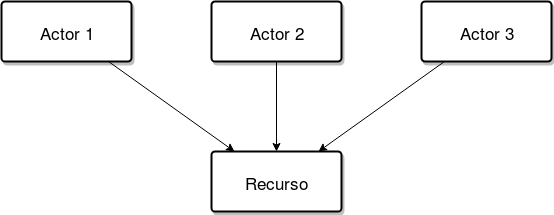
\includegraphics[width=0.85\textwidth]{./producers_only.png}
  \end{figure}
  
  \begin{itemize}
    \item \textbf{Como tenemos m\'ultiples fuentes de eventos, tenemos \textexclamdown muchos! problemas de concurrencia}
  \end{itemize}

\end{frame}


\subsection{Cola de Eventos (Event Queue)}

\begin{frame}[plain,fragile]{\textquestiondown C\'omo atenderlos a todos?}{
}
 
  \begin{itemize}

    \item Antes en el curso vimos varias t\'ecnicas para evitar problemas de concurrencia, y destacamos dos:
    \begin{enumerate}
      \item Mutex para encerrar las critical sections.
      \item Colas bloqueantes.
    \end{enumerate}

    \item Esas t\'ecnicas tienen en com\'un que serializaban cosas.
    \begin{enumerate}
      \item Usando mutex podemos ver una serializaci\'on de critical sections (se hace primero la CS que pidi\'o el mutex primero, despu\'es otra, etc).
      \item Usando colas bloqueantes, son los datos los que quedan serializados por la naturaleza FIFO de la estructura.
    \end{enumerate}

  \end{itemize}

\end{frame}

\begin{frame}[plain,fragile]{\textquestiondown C\'omo atenderlos a todos?}{
}
  \begin{itemize}

    \item Podemos modelizar a los eventos como estructuras de datos.

    \item Los eventos son producidos por m\'ultiples actores (como los que mencionamos antes).

    \item Y luego son agregados a una cola para que alguien los atienda.

  \end{itemize}

\end{frame}

\begin{frame}[plain,fragile]{Event Queue}{
}

  \begin{figure}
    \centering
    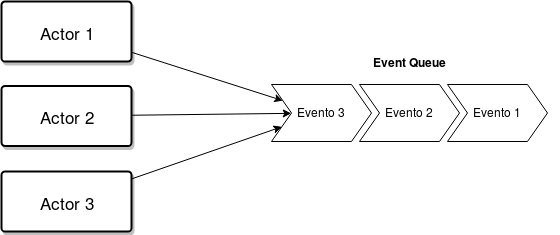
\includegraphics[width=0.85\textwidth]{./producers_to_queue.png}
  \end{figure}

  \begin{itemize}

    \item A esa cola la llamaremos \textbf{cola de eventos} (\textbf{event queue}).

    \item Protegiendo la cola de eventos ya no tenemos problemas de concurrencia. \textquestiondown Por qu\'e?

  \end{itemize}

\end{frame}


\subsection{Bucle de Eventos (Event Loop)}

\begin{frame}[plain,fragile]{\textquestiondown Qui\'en lee los eventos de la cola?}{
  Un pseudoc\'odigo para manejar eventos
}

  \begin{lstlisting}[style=normal,firstnumber=1]
while se debe continuar:
  evento := obtener el siguiente elemento de la cola de eventos
  
  if evento == salir:
    se debe continuar := false

  else if existe manejador para evento:
    ejecutar manejador

  \end{lstlisting}

  \begin{itemize}

    \item A este bucle se lo llama \textbf{event loop} y es un patr\'on muy usado en aplicaciones con \textit{Graphical User Interfaces (GUIs)}.

    \item Es similar al \textbf{game loop} que usan los juegos para simular el paso del tiempo.

  \end{itemize}

\end{frame}

\begin{frame}[plain,fragile]{Event Loop}{
  Actualizando nuestro diagrama...
}

  \begin{figure}
    \centering
    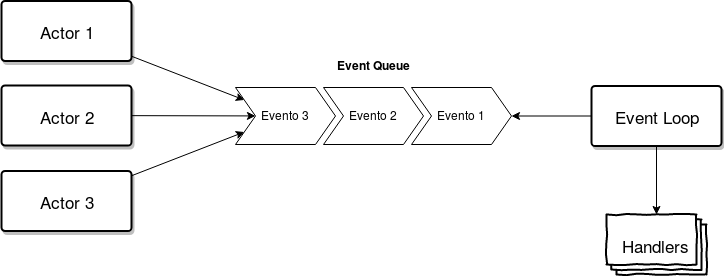
\includegraphics[width=0.85\textwidth]{./producers_to_queue_to_loop.png}
  \end{figure}

  \begin{itemize}

    \item A esa cola la llamaremos \textbf{cola de eventos} (\textbf{event queue}).

    \item Protegiendo la cola de eventos ya no tenemos problemas de concurrencia. \textquestiondown Por qu\'e?

  \end{itemize}

\end{frame}


\subsection{Manejadores (Handlers)}

\begin{frame}[plain,fragile]{Handlers}{
}

  \begin{itemize}
    \item Los \textbf{handlers} son secciones de c\'odigo que saben c\'omo responder a la aparici\'on de un Evento.

    \item Pueden requerir cierta informaci\'on sobre el Evento (en qu\'e coordenadas de la pantalla se hizo un click, cu\'anto dur\'o la pulsaci\'on de un bot\'on, alguna informaci\'on que decida el usuario).

    \item Como los va a disparar el event loop, se van a ejecutar de manera secuencial:
    \begin{itemize}
      \item No van a tener problemas de concurrencia entre ellos.
      \item Si uno tarda mucho, va a retrasar a todos los que vengan despu\'es.
    \end{itemize}

  \end{itemize}

\end{frame}

\begin{frame}[plain,fragile]{Handlers en aplicaciones con GUI}{
}

  \begin{itemize}

    \item \textbf{En aplicaciones con GUI tenemos que programar handlers cortos, y que den feedback al usuario.}

    \item Si el usuario pide alg\'un procesamiento largo conviene pasarle la tarea a alg\'un thread (ya sea lanz\'andolo o no), decirle al usuario que se est\'a procesando su pedido, y terminar el handler para que el event loop siga adelante.

    \item En muchos frameworks gr\'aficos, el event loop corre en el hilo principal.
    \begin{itemize}
      \item Algunos nos abstraen de programarlo (como GTK).
      \item En otros lo tenemos que programar nosotros (como SDL).      
    \end{itemize}

  \end{itemize}

\end{frame}


\section{Conclusiones}

\begin{frame}[plain,fragile]{Conclusiones}{
}

  \begin{itemize}

    \item La programaci\'on orientada a eventos nos evita los problemas de concurrencia entre los handlers.

    \item Es un paradigma muy usado para interactuar con el usuario, ya que es \'el qui\'en decide el flujo del programa.

    \item Cuando hay GUI, como los handlers se ejecutan secuencialmente conviene programarlos cortos y delegar las tareas largas en otro hilo.

    \item Es casi esencial el multithreading cuando tenemos GUIs, y el loop de eventos suele correr en el hilo principal.

  \end{itemize}

\end{frame}


\section{Temas Relacionados}

\begin{frame}[plain,fragile]{Temas (muy) relacionados}{
}
  \begin{itemize}

    \item Muchos frameworks trabajan con event queues y nos abstraen de su uso.
    \begin{enumerate}
      \item En C/C++, podemos mencionar a QT y GTK+ (o gtkmm), que usan una event queue para manejar las interacciones con el usuario. Veremos una de estas opciones la clase que viene.
      \item En otros lenguajes, NodeJS basa TODO en una event queue.
    \end{enumerate}

    \item Este patr\'on es muy parecido al Observer (pero con un poco menos de acoplamiento).

    \item En abstracto, el concepto es el mismo que el de una \textit{cola de mensajes}, o un \textit{publish/subscribe}, pero el t\'ermino que usamos depende del contexto.

    \item Varios lenguajes de programaci\'on, como Go implementan \textbf{channels} (nombre en Go) nativos, que son en esencia event queues o message queues.

  \end{itemize}

\end{frame}

\end{document}
